%!TEX root = ../main.tex

\subsection{The Role of Acceleration and other Algorithmic Components}\label{app:acceleration-exps}

\begin{figure}
	\centering
	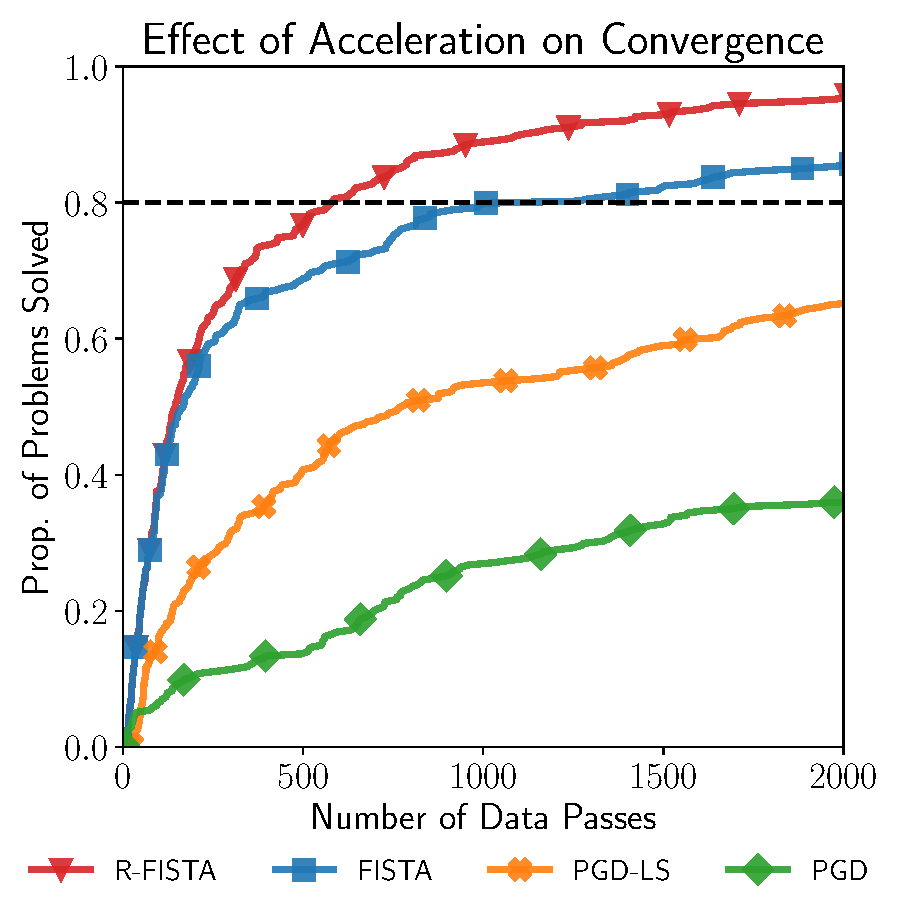
\includegraphics[width=0.95\linewidth]{figures/chapter_two/pp_acceleration.pdf}
	\caption{Performance profile comparing R-FISTA, FISTA without restarts, proximal gradient descent with line-search (PGD-LS) and proximal gradient descent with a fixed step-size (PGD) for solving C-GReLU on 73 datasets from the UCI repository.
		For PGD, we report results for the best step-size chosen by grid-search individually for each problem.
		R-FISTA solves a higher proportion of problems in fewer passes through the dataset.
	}%
	\label{fig:acceleration-pp}
\end{figure}

This section studies the effects of different algorithmic components on the optimization performance of R-FISTA for the C-GReLU problem.
By systematically removing restarts, acceleration, and line-search, we illustrate the importance of these enhancements to the speed and robustness of the optimization procedure.

\cref{fig:acceleration-pp} shows a performance profile comparing R-FISTA, the FISTA algorithm without restarts (FISTA), proximal gradient descent with the line-search described in Section~\ref{sec:efficient-fista} (PGD-LS), and proximal gradient descent (PGD) with a fixed step-size.
We use the same problem set as for \cref{fig:performance-profiles}: \( 438 \) individual training problems generated by considering six regularization parameters for \( 73 \) datasets taken from the UCI dataset repository.
See \cref{app:uci-datasets} for more details.
Note that we do not include problems for which the regularization parameter is overly large and a degenerate model (ie.\ all zeros) is optimal.
A problem is considered solved the minimum norm subgradient has norm less than or equal to \( 10^{-3} \); in practice, we check an identical condition on the gradient norm squared.
The C-GReLU model is formed by sampling \( 5000 \) activation patterns.

The x-axis shows the number of passes through that dataset that each method performs.
This quantity is equivalent to the iteration counter for PGD; for the remaining methods it also includes the number of function evaluations due to back-tracking on the line-search condition.
For R-FISTA, FISTA, and PGD-LS, we use the step-size initialization strategy described in the main paper (see Appendix~\ref{app:step-size-initialization} for experiments studying this rule) with the standard parameters given in Appendix~\ref{app:default-parameters}.
For each problem, we use the best fixed step-size for PGD out of the grid \( \cbr{10, 1, 0.1, 0.01} \).

We make the following observations:
(i) R-FISTA requires about three-fourths as many data passes as FISTA to solve \( 80\% \) of problems, which suggests restarts allow greater adaptivity to problem structure;
(ii) acceleration is critical to solving problems quickly and PGD-LS performs poorly compared to both R-FISTA and FISTA;
(iii) PGD is very slow despite using about \( 4 \times \) more compute than the other methods.

\begin{figure}
	\centering
	\ifdefined\smallPDF
		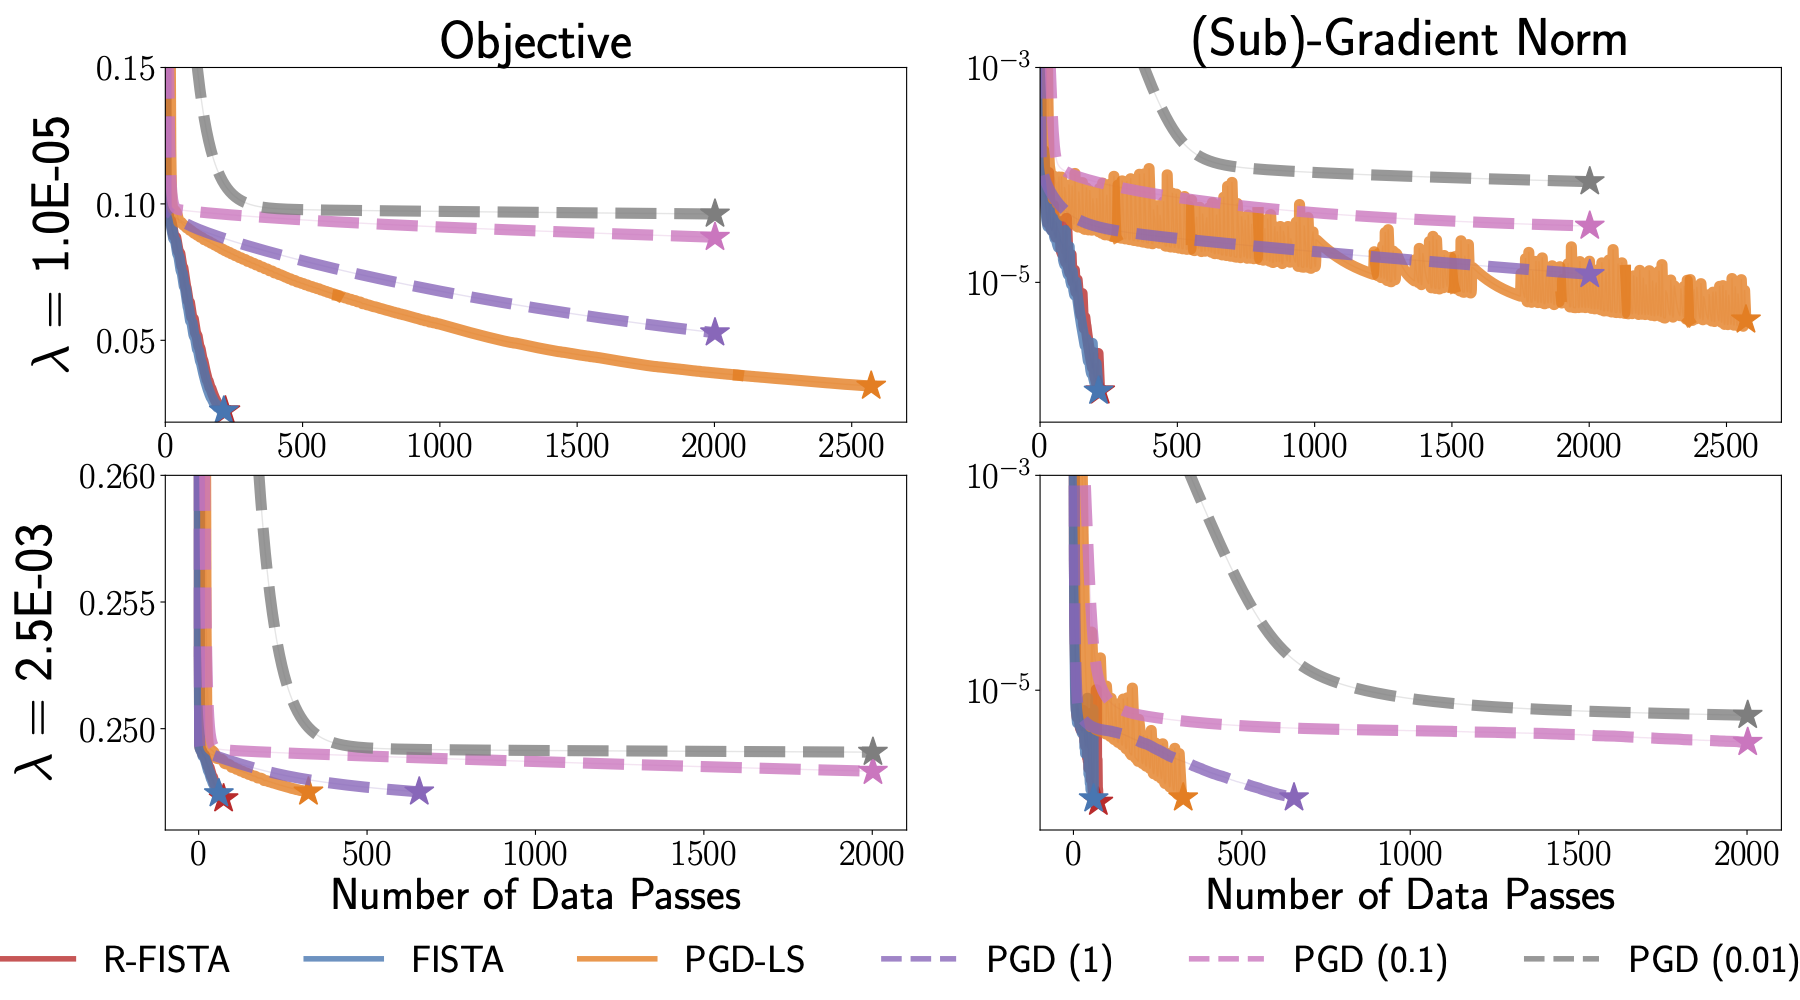
\includegraphics[width=0.95\linewidth]{figures/chapter_two/acceleration/twonorm.png}%
	\else
		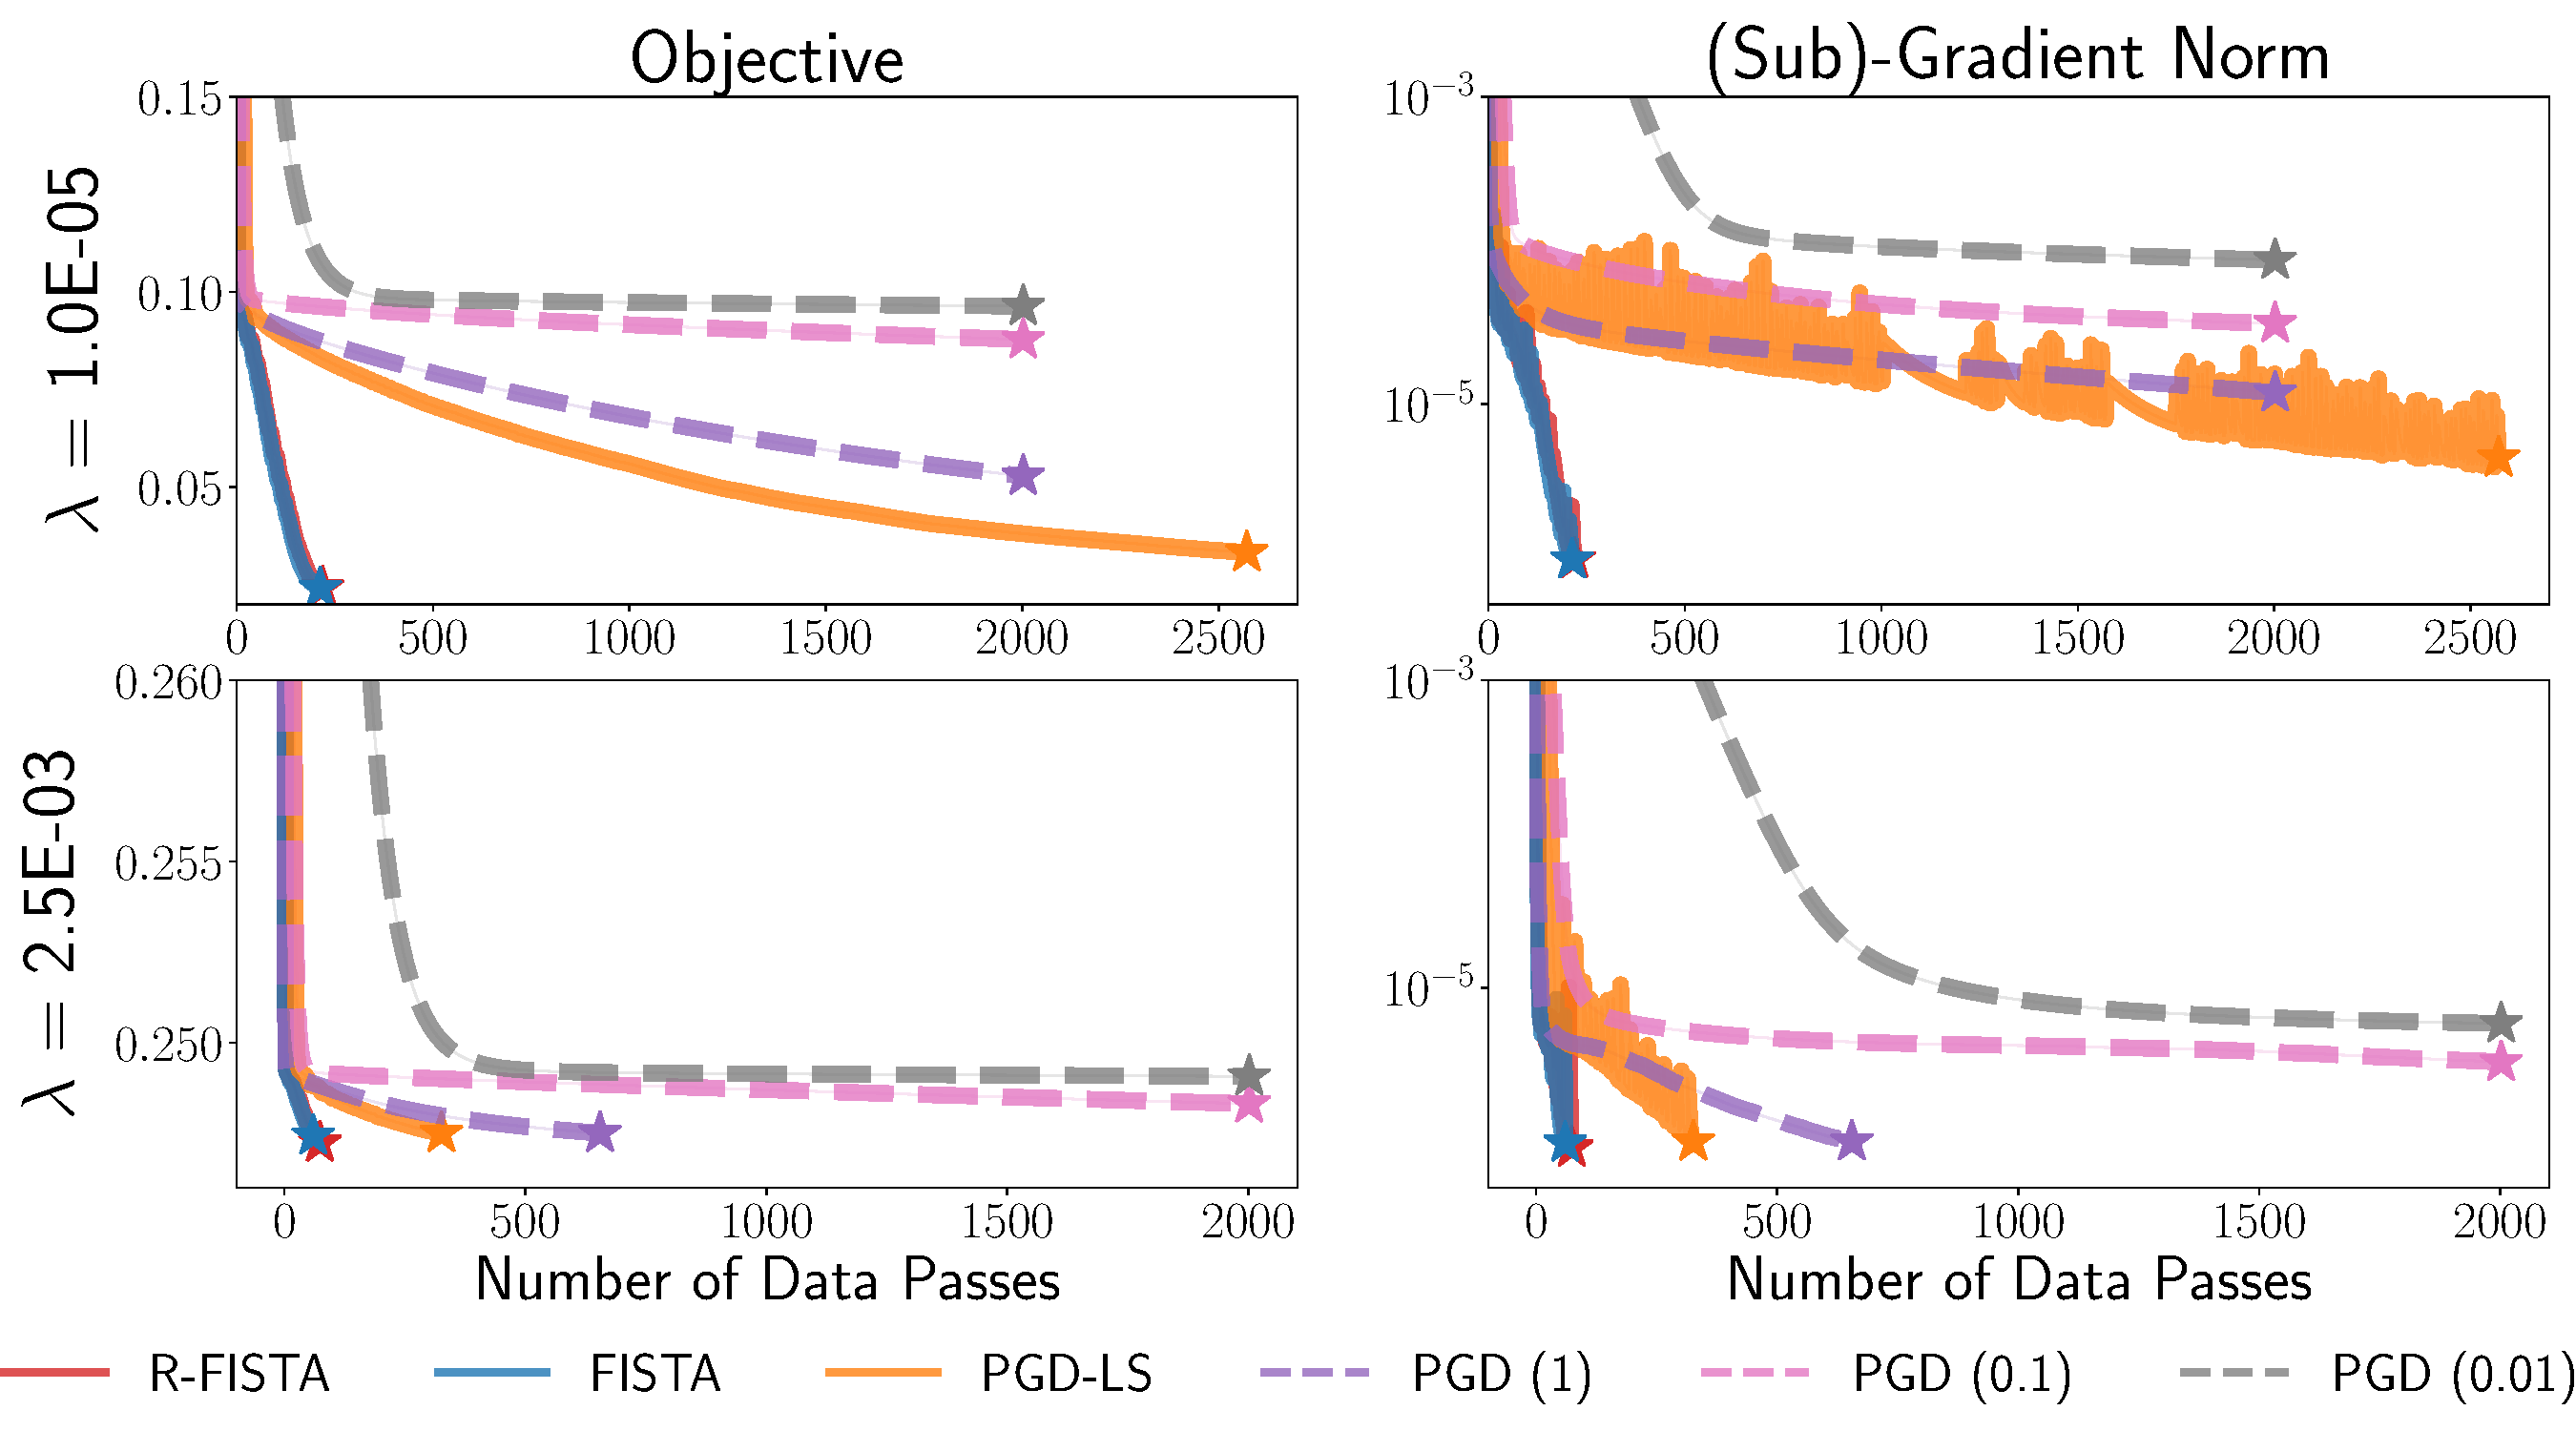
\includegraphics[width=0.95\linewidth]{figures/chapter_two/acceleration/twonorm.pdf}%
	\fi
	\caption{Convergence comparison for R-FISTA, FISTA without restarts (FISTA), proximal gradient descent with line-search (PGD-LS) and proximal gradient descent (PGD) with several fixed step-sizes (reported in parenthesis) on the \texttt{twonorm} dataset.
		PGD stalls while the accelerated methods converge very quickly to an approximate stationary point.
	}%
	\label{fig:acceleration-twonorm}
\end{figure}


\begin{figure}
	\centering
	\ifdefined\smallPDF
		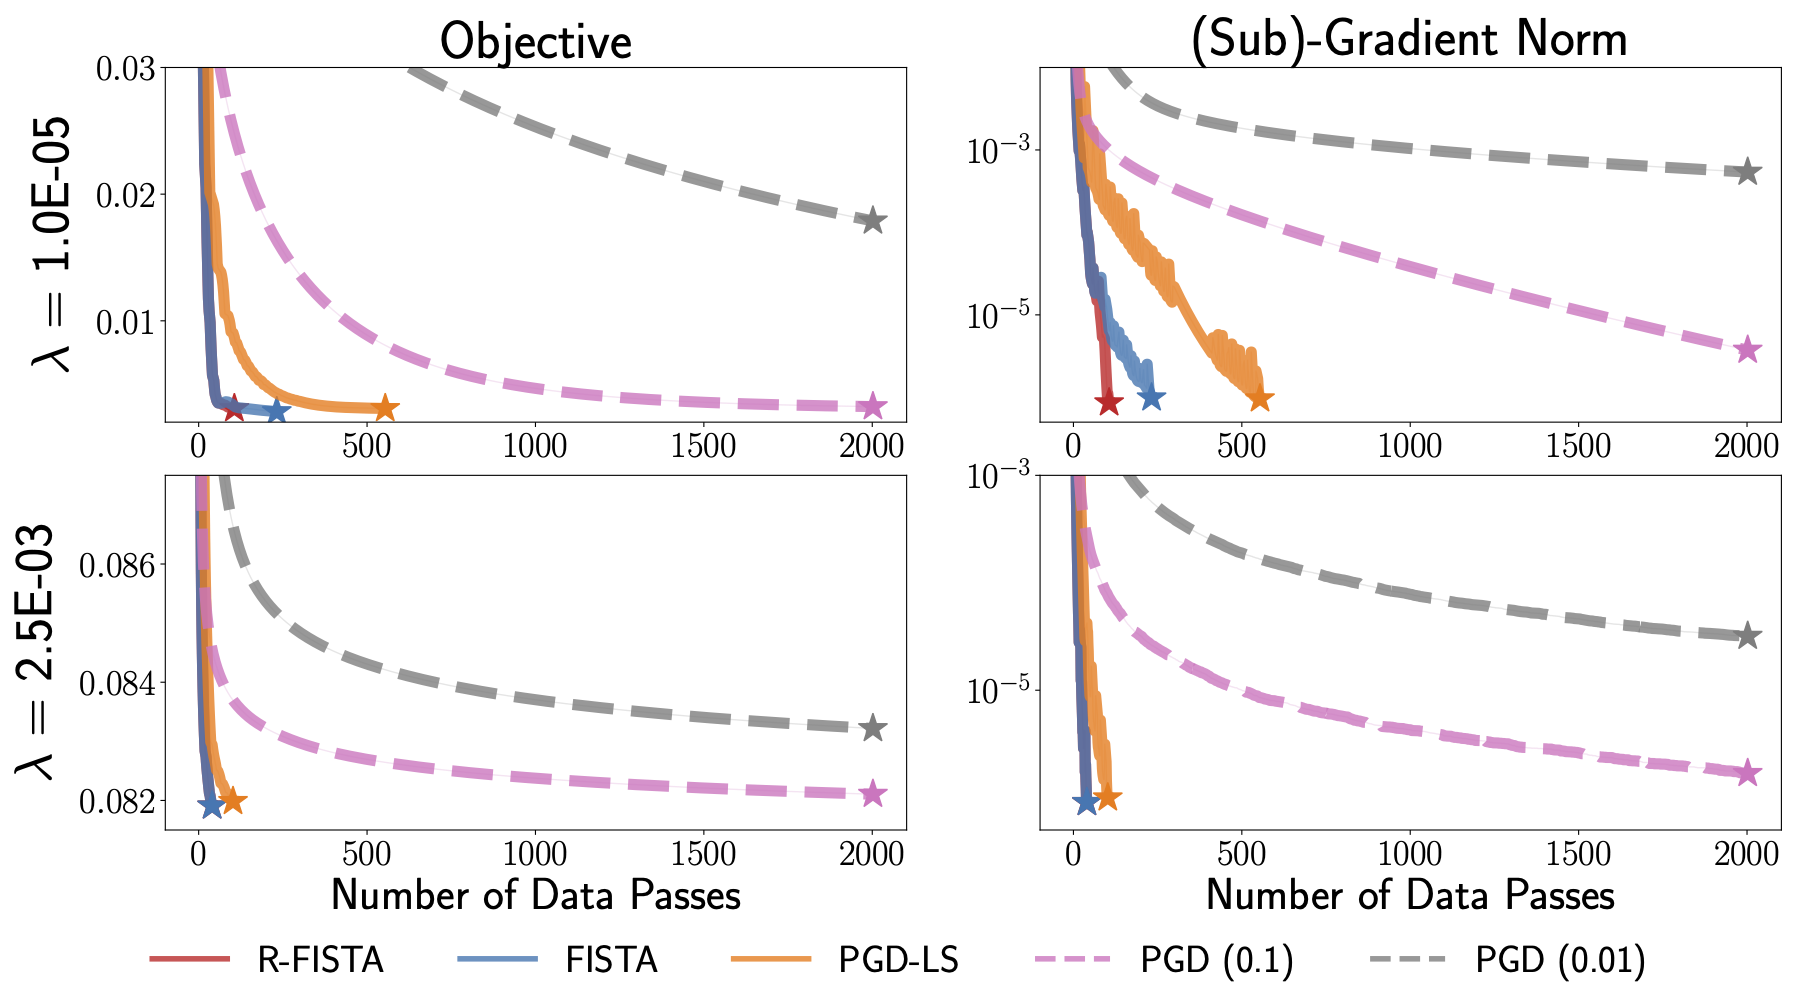
\includegraphics[width=0.95\linewidth]{figures/chapter_two/acceleration/heart-cleveland.png}%
	\else
		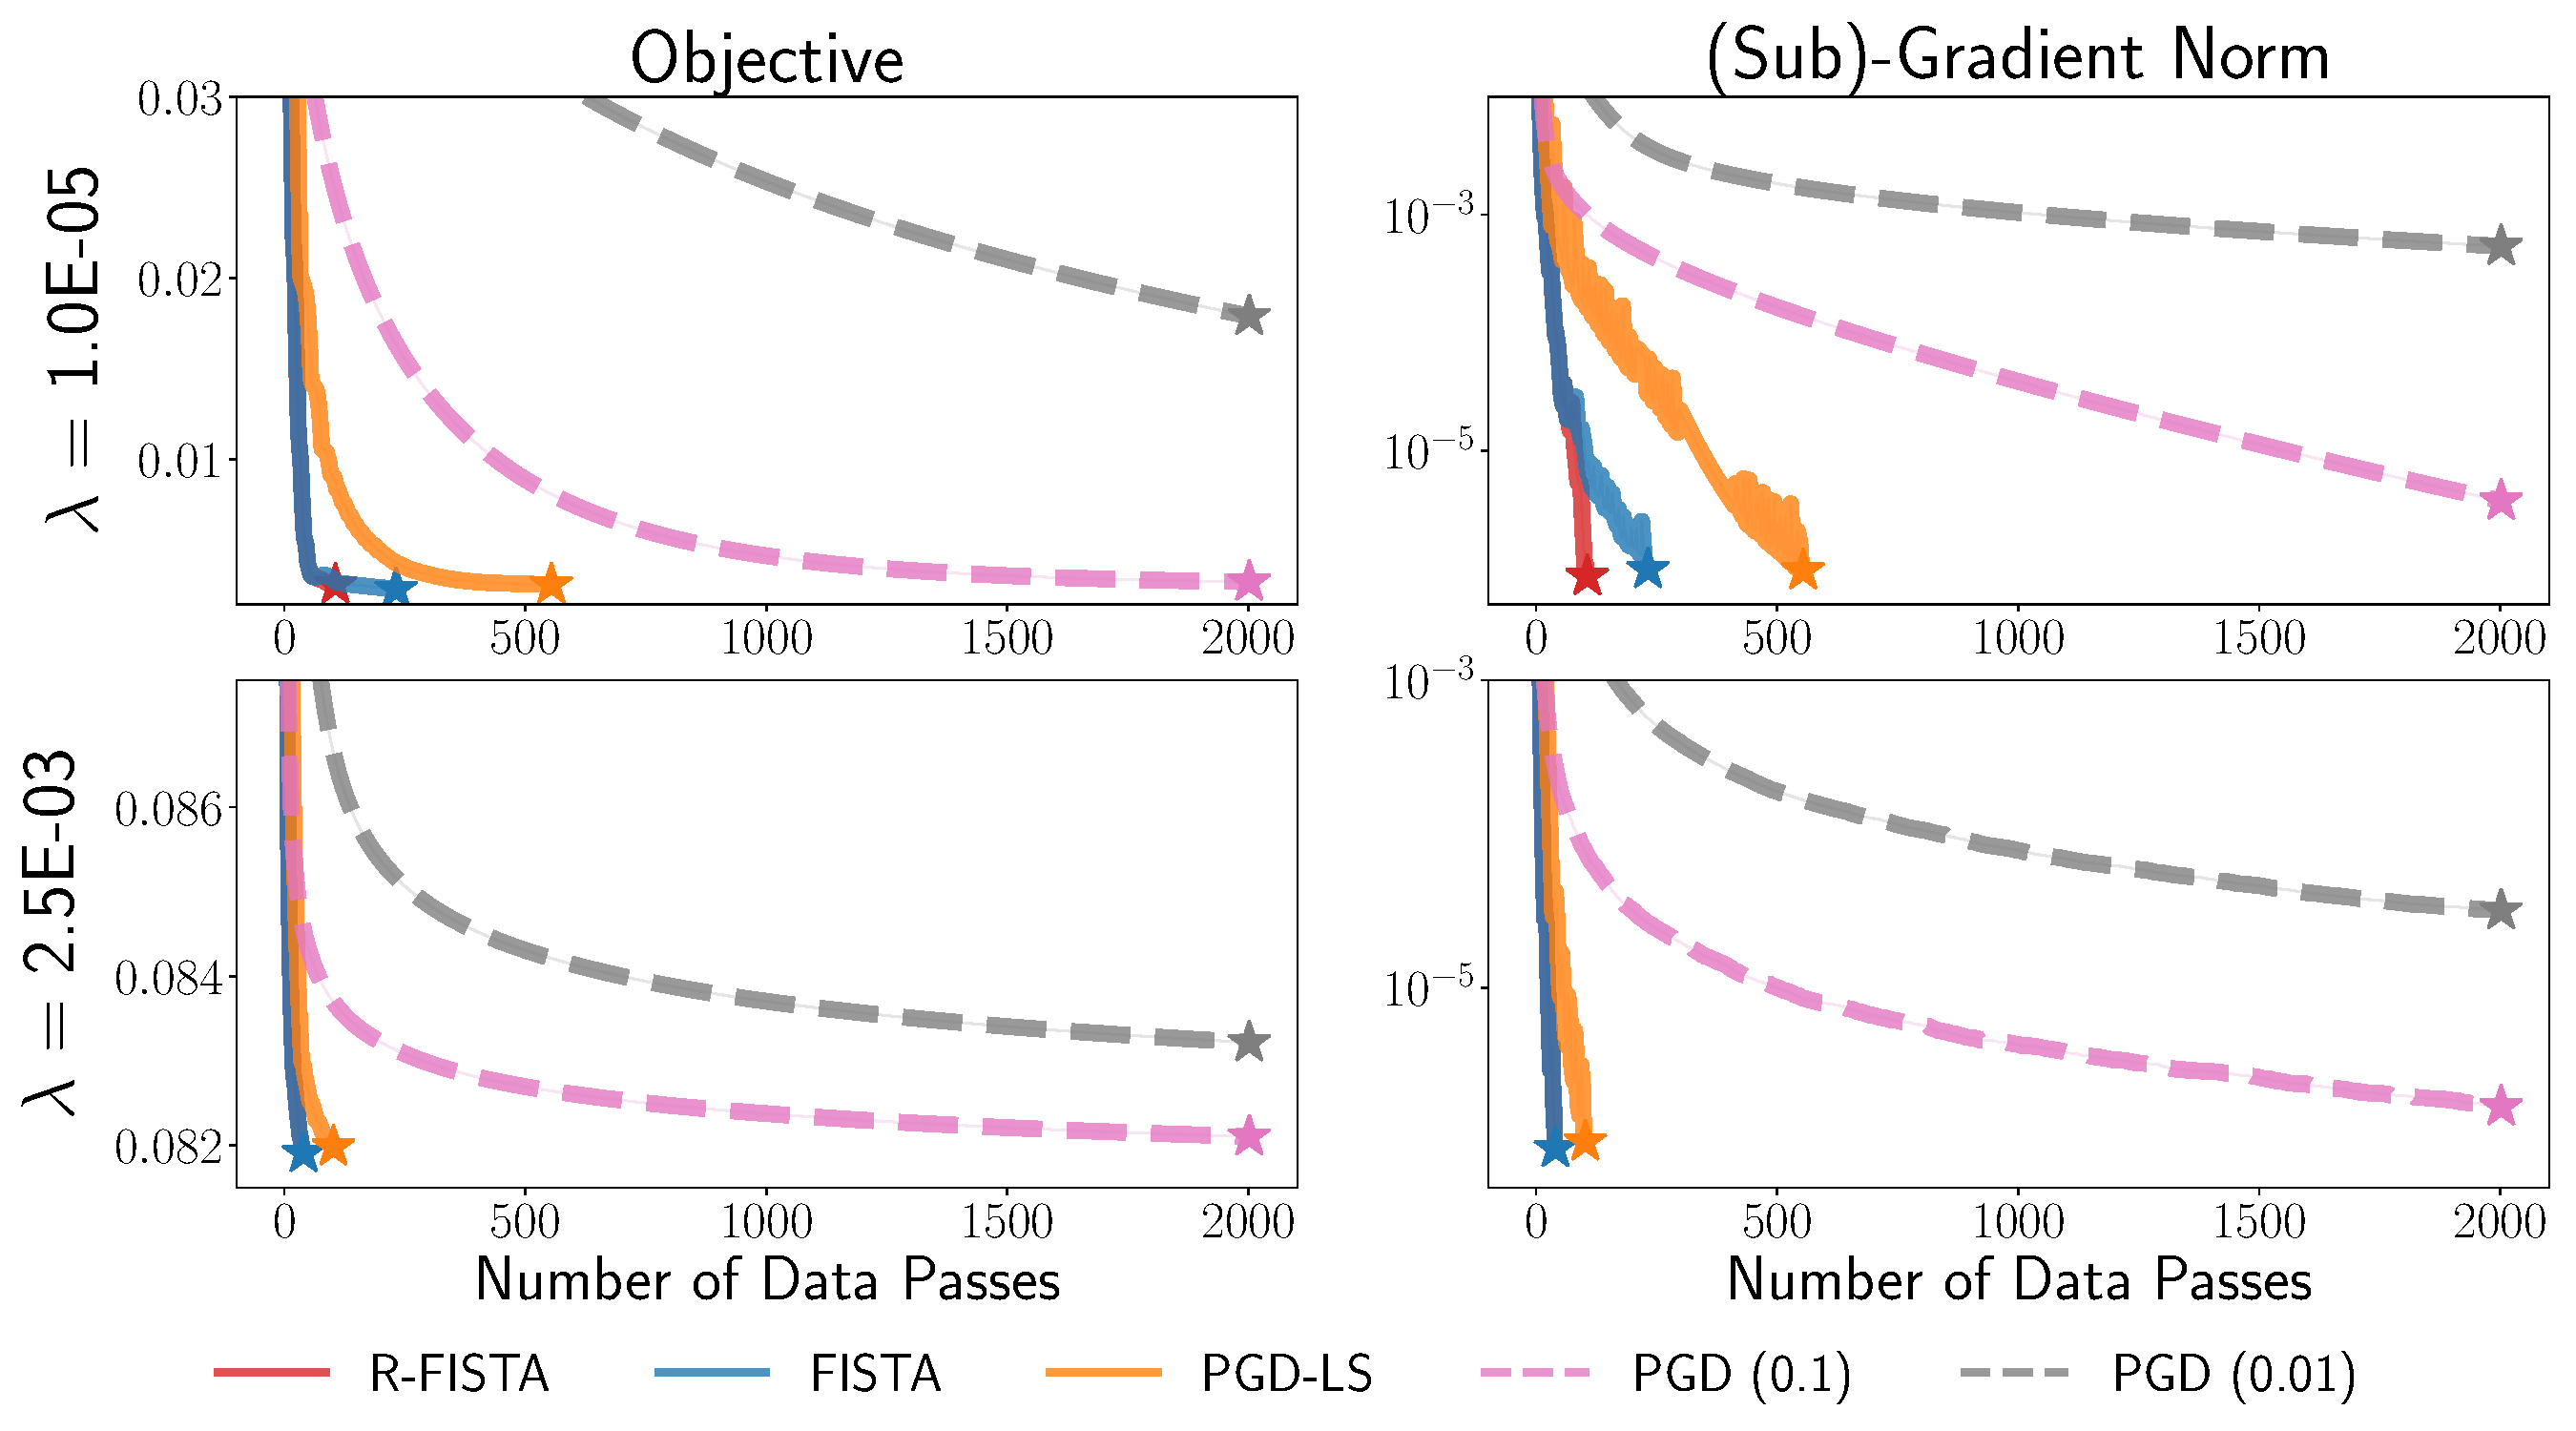
\includegraphics[width=0.95\linewidth]{figures/chapter_two/acceleration/heart-cleveland.pdf}%
	\fi
	\caption{Convergence comparison for R-FISTA, FISTA without restarts (FISTA), proximal gradient descent with line-search (PGD-LS) and proximal gradient descent (PGD) with several fixed step-sizes (reported in parenthesis) on the \texttt{heart-cleveland} dataset.
		The performance of R-FISTA and FISTA is identical when \( \lambda = 2.5 \times 10^{-3} \).
		In contrast, restarting allows R-FISTA to converge in around half as many iterations as FISTA for the smoother problem with \( \lambda = 1 \times 10^{-5} \).
	}%
	\label{fig:acceleration-heart-cleveland}
\end{figure}

We also report convergence behavior on two randomly selected datasets to illustrate the fine-grained performance of each method.
Figures~\ref{fig:acceleration-twonorm} and~\ref{fig:acceleration-heart-cleveland} show the convergence of R-FISTA, FISTA, PGD-LS, and PGD with respect to objective value and subgradient norm (squared) for the \texttt{twonorm} and \texttt{heart-cleveland} datasets.
Results for are shown for the smallest regularization parameter considered and the largest for which the model was not degenerate.
We omit step-sizes for which PGD diverged.


\subsection{Step-size Update Rules}\label{app:step-size-initialization}

\begin{figure}[t]
	\centering
	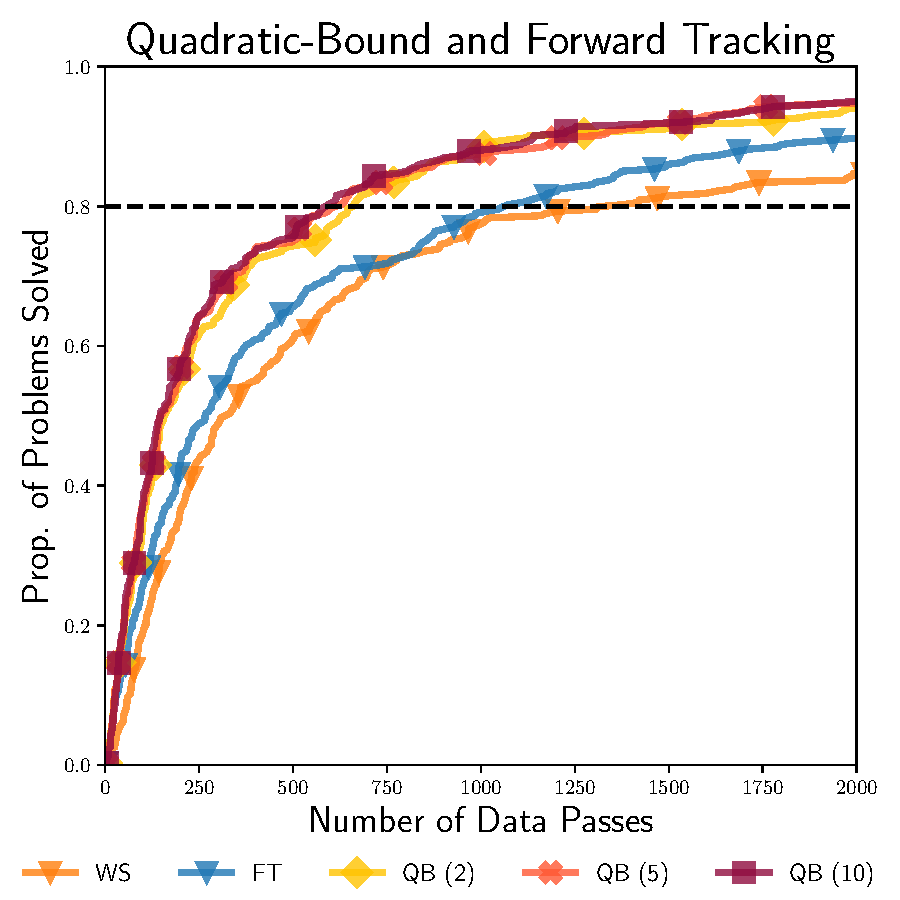
\includegraphics[width=0.8\linewidth]{figures/chapter_two/pp_lassplore.pdf}
	\caption{Performance profile comparing R-FISTA, FISTA with different step-size initialization rules.
		We compare checking the quadratic bound for tightness (QB) with a variety of choices for the threshold parameter \( c \) against warm starting as \( \etak = \eta_{k-1} \) (WS), and forward tracking (FT).
		As before, we generate the profile by solving the C-GReLU problem on 73 datasets from the UCI repository.
		QB is robust to the choice of \( c \) and outperforms both WS and FT.
		WS and FT have similar performance despite very different behavior.
	}%
	\label{fig:lassplore-pp}
\end{figure}


Now we perform an ablation study on the step-size initialization rule proposed by \citet{liu2009lassplore} and discussed in Section~\ref{sec:efficient-fista}.
Throughout this section, we refer to this initialization strategy as quadratic-bound (QB).
We compare QB against warm starting as \( \etak = \eta_{k-1} \) (WS), and forward tracking (FT).
As in the previous section, we use a performance profile to summarize results for solving the C-GReLU problem on the same \( 438 \) problems as in \cref{fig:performance-profiles}.
We use the same backtracking parameter \( \beta = 0.8 \) for QB, WS, and FT, while we use a forward-tracking parameter of \( \alpha = 1.25 \) for QB and FT.
Note that these are the standard parameters discussed in Appendix~\ref{app:default-parameters}.
We use the standard settings for all other parameters of R-FISTA.
We sample \( 5000 \) random activation patterns just as in the previous section.

Empirically, we find (see Figure~\ref{fig:lassplore-pp}) that the QB initialization strategy is surprisingly resilient to the choice of threshold parameter, \( c \).
Indeed, QB with any \( c \in \cbr{10, 5, 2} \) is more efficient than FT or WS.
Surprisingly, FT and WS have similar performance despite their substantially different convergence behavior (see Figures~\ref{fig:lassplore-glass} and~\ref{fig:lassplore-flags}).
This is primarily because we measure progress in total data passes, which includes the unnecessary backtracking performed by R-FISTA with the FT update.



\begin{figure}
	\centering
	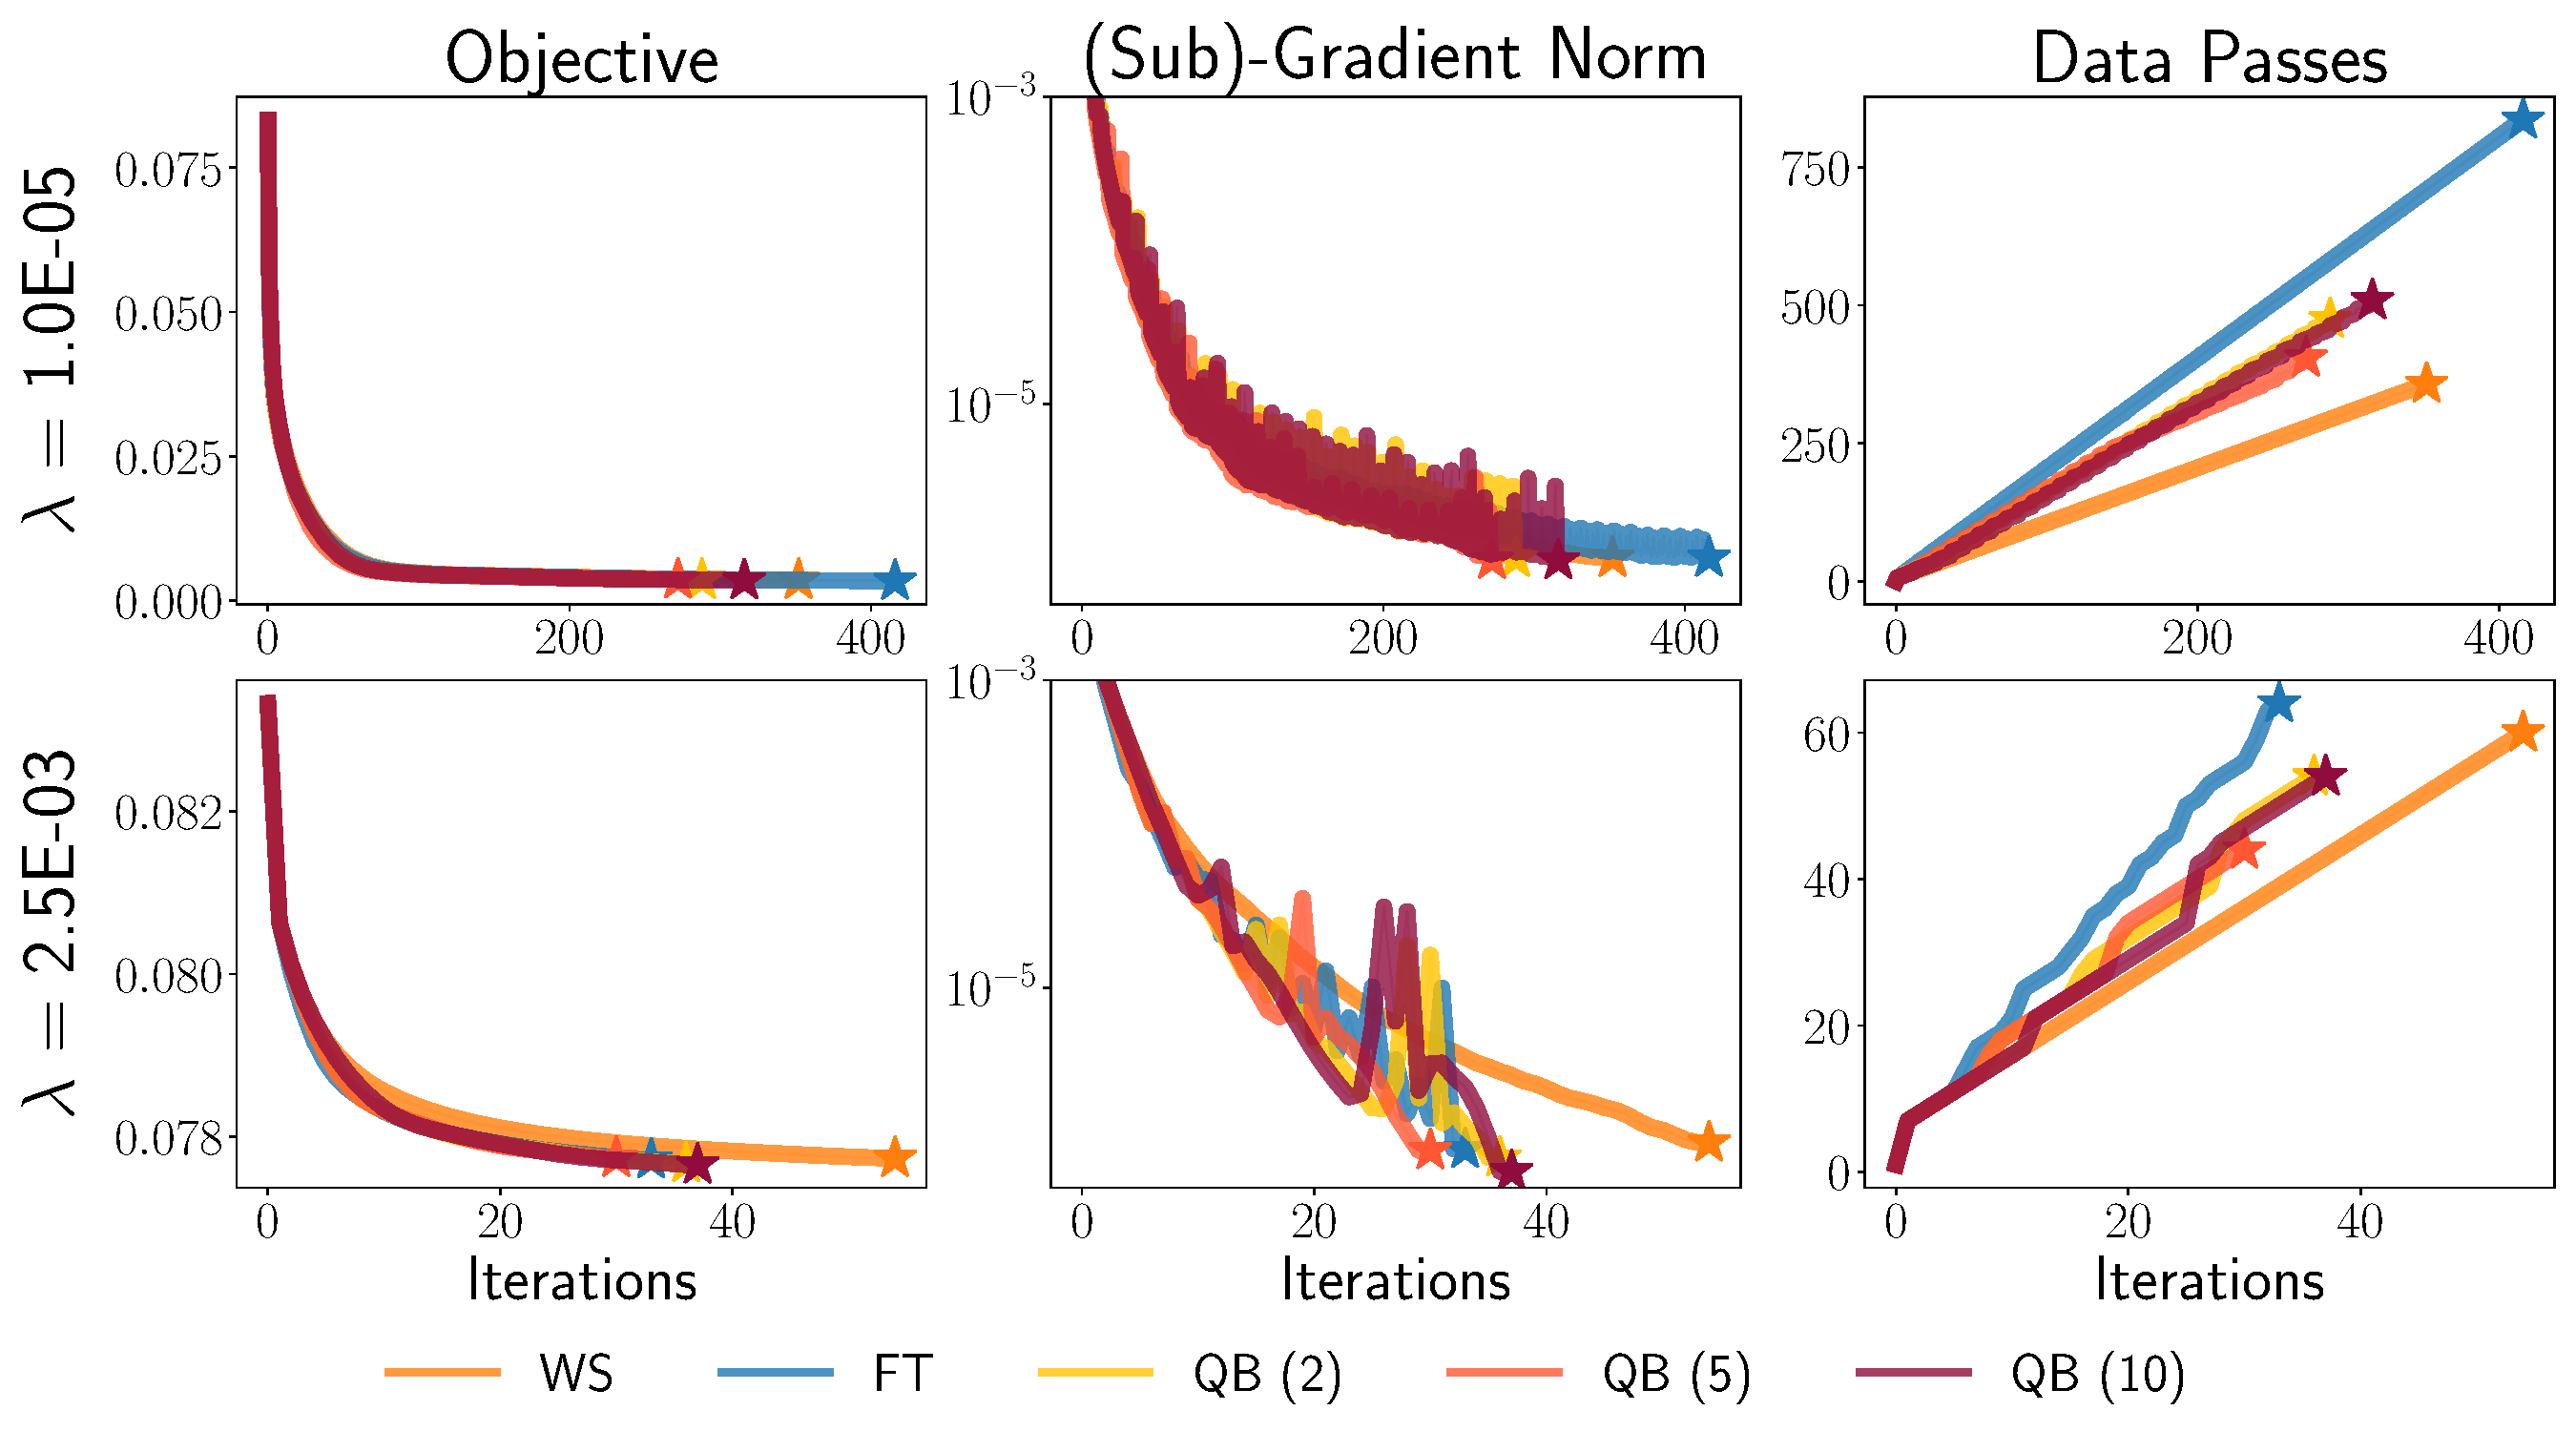
\includegraphics[width=0.95\linewidth]{figures/chapter_two/lassplore/glass}
	\caption{Convergence of R-FISTA with different step-size initialization rules on the \texttt{glass} dataset.
		We compare warm-starting (WS) and forward-tracking (FT) against the initialization proposed by \citet{liu2009lassplore} (QB) for several fixed thresholds (reported in parentheses).
		QB has similar convergence performance to FT without requiring as many passes through the training set and is resilient to the choice of threshold.
	}

	\label{fig:lassplore-glass}
\end{figure}

\begin{figure}
	\centering
	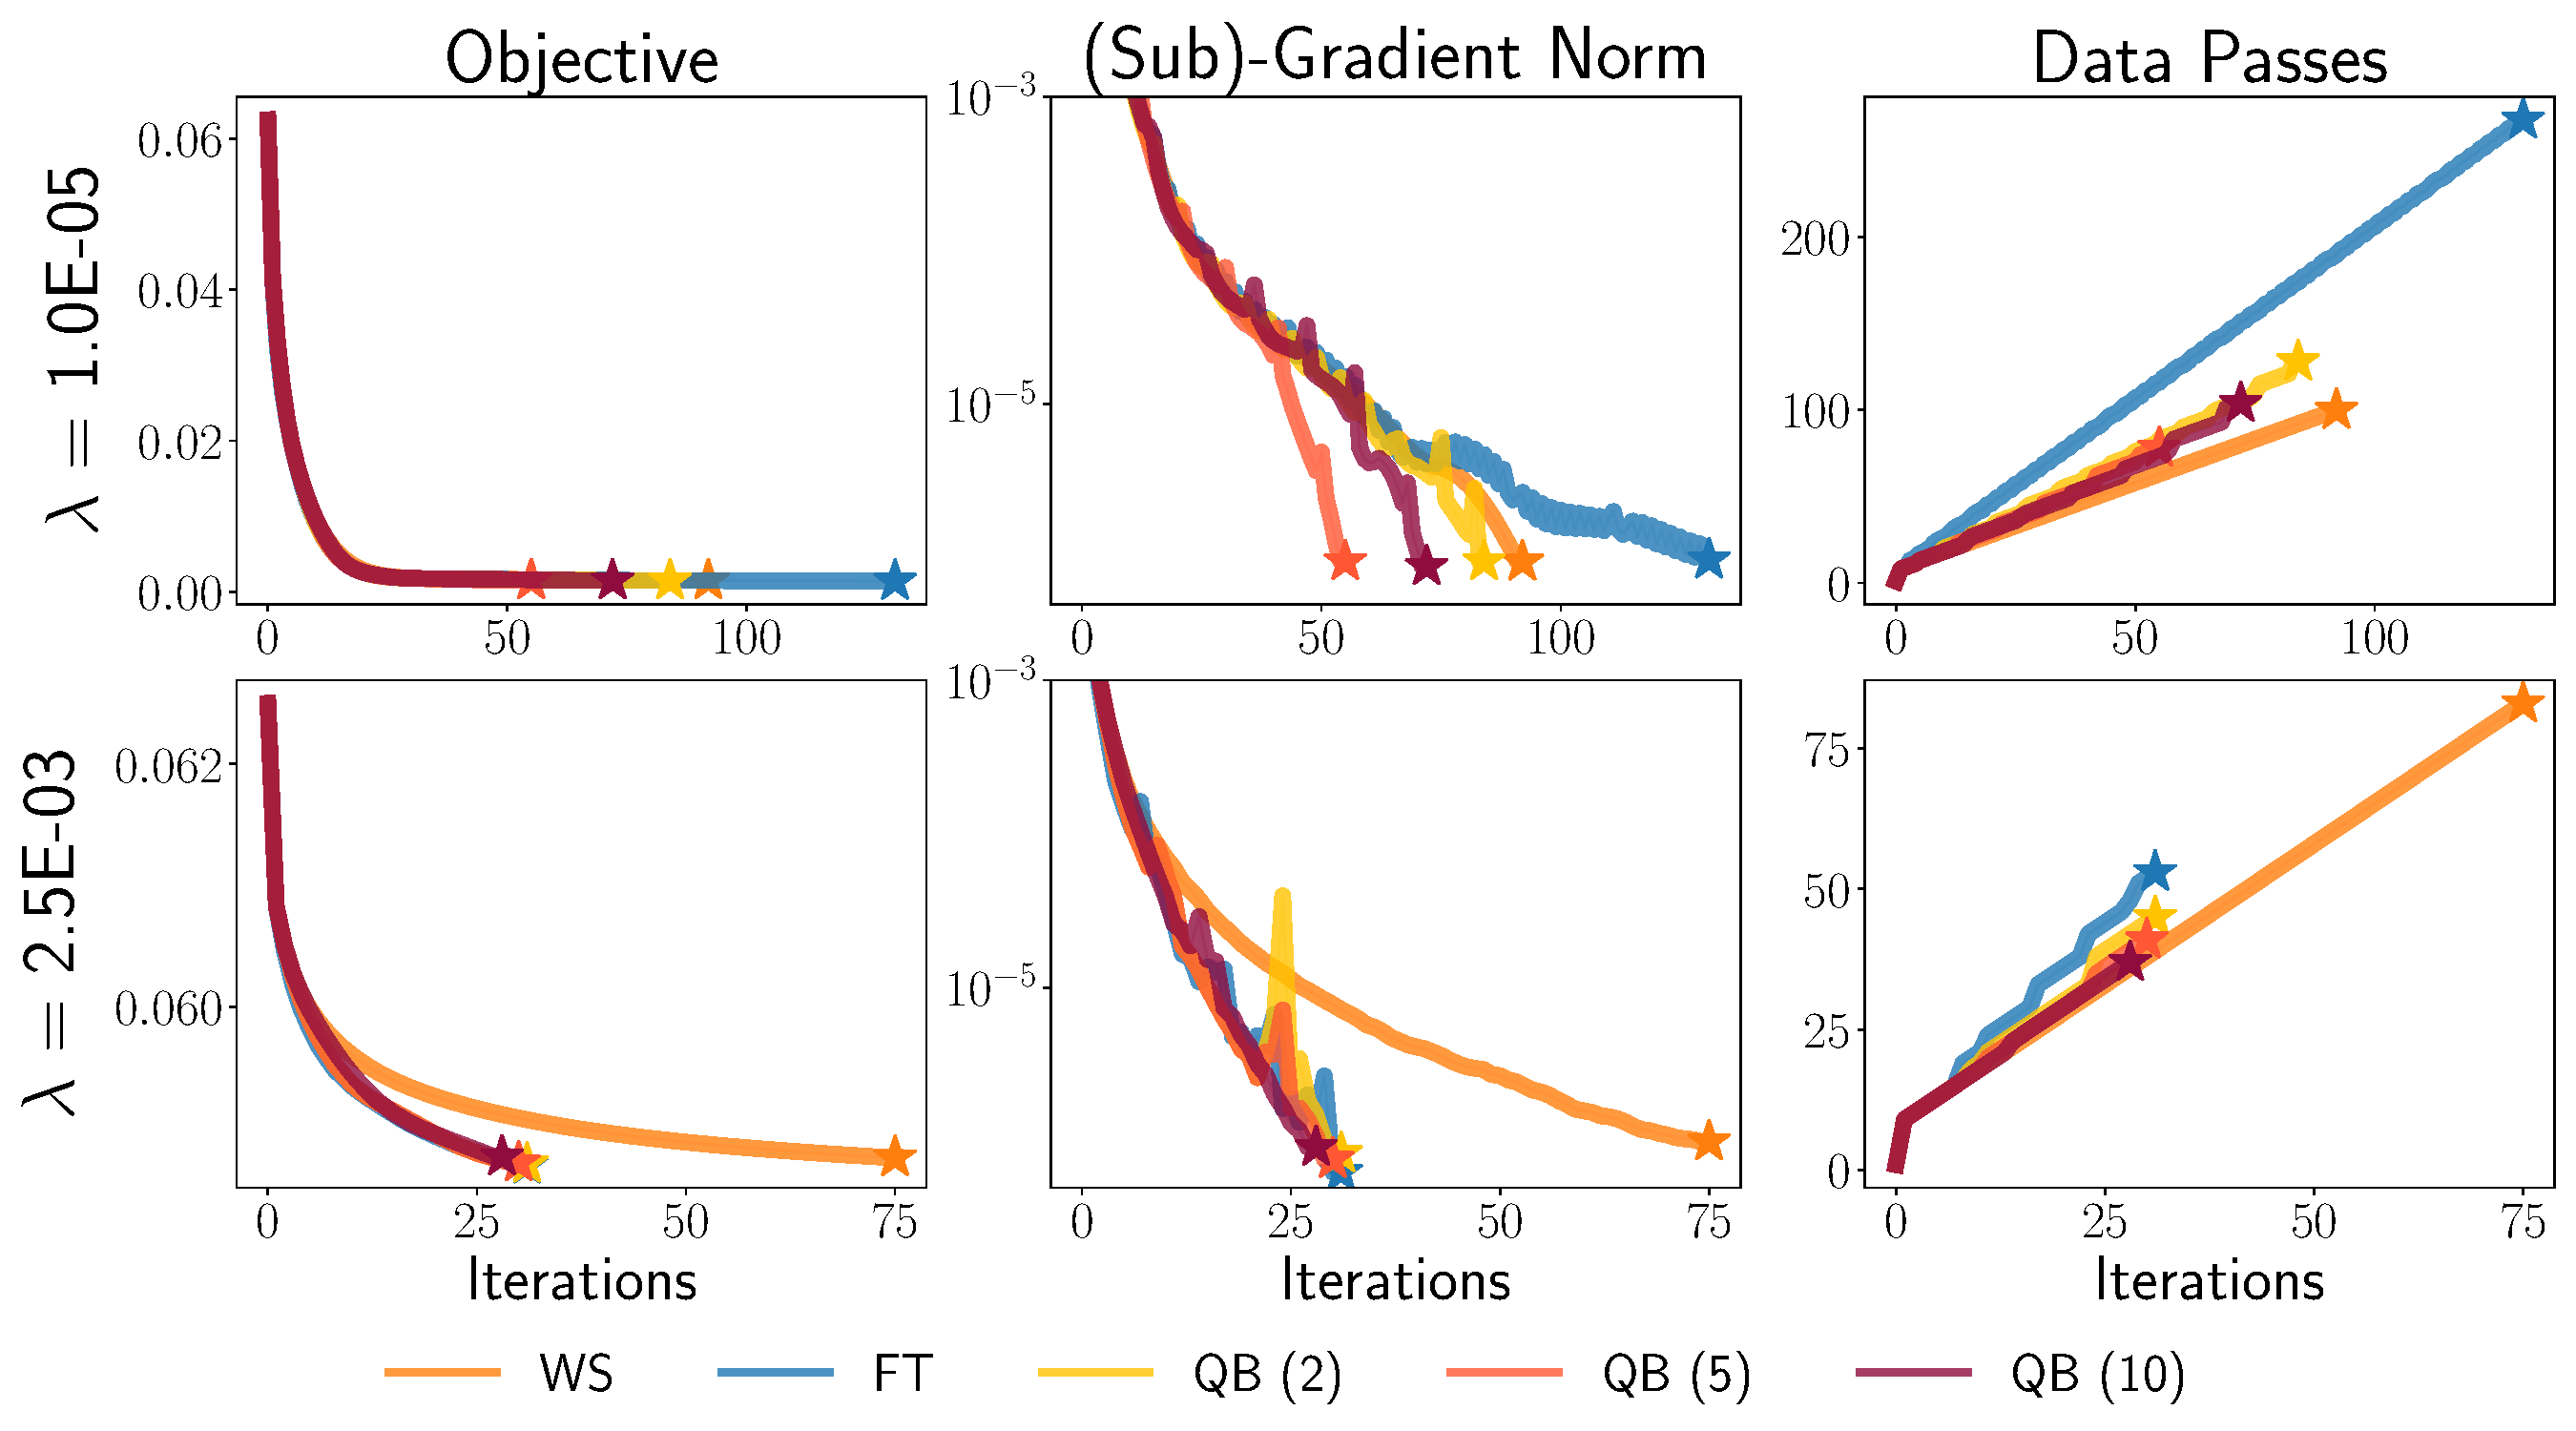
\includegraphics[width=0.95\linewidth]{figures/chapter_two/lassplore/flags}
	\caption{Convergence of R-FISTA with different step-size initialization rules on the \texttt{flags} dataset.
		See \cref{fig:lassplore-glass} for additional details.}%
	\label{fig:lassplore-flags}
\end{figure}
